\documentclass[
	%draft,
	%submission,
	%compressed,
	final,
	%
	%technote,
	%internal,
	%submitted,
	%inpress,
	%reprint,
	%
	%titlepage,
	notitlepage,
	%anonymous,
	narroweqnarray,
	inline,
	twoside,
         %invited,
	]{ieee}

\newcommand{\latexiie}{\LaTeX2{\Large$_\varepsilon$}}

%Code
	\usepackage{listings}
	\usepackage{fancyvrb}
	\usepackage{moreverb}
	\usepackage{listings}
%	\DefineVerbatimEnvironment{code}{Verbatim}{fontsize=\small}
%	\DefineVerbatimEnvironment{example}{Verbatim}{fontsize=\small}
	\usepackage{amssymb}
	\def\myTabs{2}
%edoC
\usepackage{graphicx}
%Español
	\usepackage[utf8]{inputenc}
	\usepackage[spanish]{babel}
%loñapsE

\begin{document}

\title[Load Balancer]{
       Telemática\\ Load Balancer}


\author[]{Sebastián Arcila Valenzuela (\textit{sarcilav@eafit.edu.co})
\and{}y Sergio Botero Uribe (\textit{sbotero2@eafit.edu.co}).
}

\journal{ST0255-031 Telemática}
\titletext{, \today}
\maketitle               

\begin{abstract} 
Documentación de la práctica del load balancer para servidores web que implementa 4 métodos de balanceo. Esta documentación
contiene los diagramas requeridos para la entrega y la explicación de los métodos.
\end{abstract}

\section{Introducción}
	%%introducción
Los métodos de balanceo de cargas surgen como la solución para equilibrar el trabajo realizado por cualquier unidad que forme parte de un grupo
que trata de prestar un servicio como uno solo. El balanceo de carga se usa en discos duros, procesadores, redes, donde para el caso de los
procesadores, la unidad que tiene menor número de tareas o que tiene más capacidad para asumir otra tarea obtiene el trabajo siguiente.
Los criterios para determinar quien debe recibir esa nueva tarea se determina mediante algún método preestablecido, de los cuales el más sencillo es
el método de Round Robin.
En la práctica el objetivo era implementar uno de estos balanceadores de carga para un grupo de servidores web, en donde la carga son las peticiones
a los recursos que se encuentran replicados en este grupo con la implementación de cuatro métodos diferentes para solucionar este problema. Los
métodos implementados son el Round Robin, menor número de conecciones actuales, menor carga en servidor y por último un método propio
propuesto por el grupo.
Los pasados métodos de balanceo se encuentran explicados y acompañados de un seudo código sencillo en este documento.
Más adelante se explica también la forma en que se opera el balanceador de carga implementado y bajo que condiciones se pueden obtener los
resultados deseados.


\section{Protocolos implementados}
	Los protocolos usados en este balanceador de carga son TCP para toda la conexión entre los clientes y el balanceador de carga, también es TCP entre
el load balancer y los servidores finales.\\
Se requirió la implementación de un protocolo para el manejo y envío de mensajes entre los agentes que residen en los servidores y el balanceador
 de cargas. Los mensajes que se intercambiarán determinan el tipo información que maneja el agente.\\
 
 Protocolo Balanceador de Carga-Agente
 
 \begin{itemize}
 \item Definición y especificaciones del protocolo.\\
El servicio que presta este protocolo es el de envío de mensajes entre el agente que está siendo ejecutado en un servidor y el balanceador de carga.
El fin de este servicio es que el balanceador pueda disponer de información sobre el servidor y sus procesos en las veces que sea necesario hasta
obtener un servidor que sea buen candidato para recibir la petición.\\
El balanceador de carga sabe que puede encontrar a cualquier agente disponible en el puerto nueve mil (9000) de cualquiera de los servidores
que puede usar para realizar el equilibrio de las peticiones.
Por estar soportados en TCP, este protocolo no se preocupa por pérdida de información, ordenamiento u otros.
  \item Suposiciones del entorno.\\
  Las condiciones ideales para el funcionamiento del protocolo serían las siguientes:
  \begin{enumerate}

\item Para el correcto funcionamiento del protocolo y de los agentes, las máquinas que los ejecuten deben estar corriendo sobre un sistema operativo
Linux, ya que la información que se toma de cada servidor se toma con comandos especiales de este sistema operativo.

\item Los puertos 9000 de cada máquina que hace parte del grupo de servidores que está siendo equilibrados en carga deben estar disponibles
para poder que el agente se ejecute sobre él. El agente necesita el puerto 9000 sólo para recibir las peticiones del balanceador.

\end{enumerate}

   \item Vocabulario de mensajes.\\
   Los mensajes enviados desde el balanceador al agente son:``lc'' y ``lbs''. Y para cada uno hay una respuesta por parte del balanceador que consiste
   en un string de tres números, del cual sólo importa el primero, y un valor flotante indicando carga del procesador respectivamente.
   ``lc'' representa el método de balanceo por menor número de conexiones activas. y ``lbs'' es el método del servidor con la menor carga o
   ``Least Busy Server''
    \item Codificación o formato de mensajes.\\
    Los mensajes se querían implementar lo más cortos posibes, por eso, para pedir una respuesta que pueda ser usada en un método de menor número
    de conexiones se debe enviar al agente la palabra ``lc''
     \item Reglas de procedimiento.\\
 \end{itemize}

\section{Diagrama de secuencias UML}
	%
%\begin{figure}[htbp] %  figure placement: here, top, bottom, or page
%   \centering
%   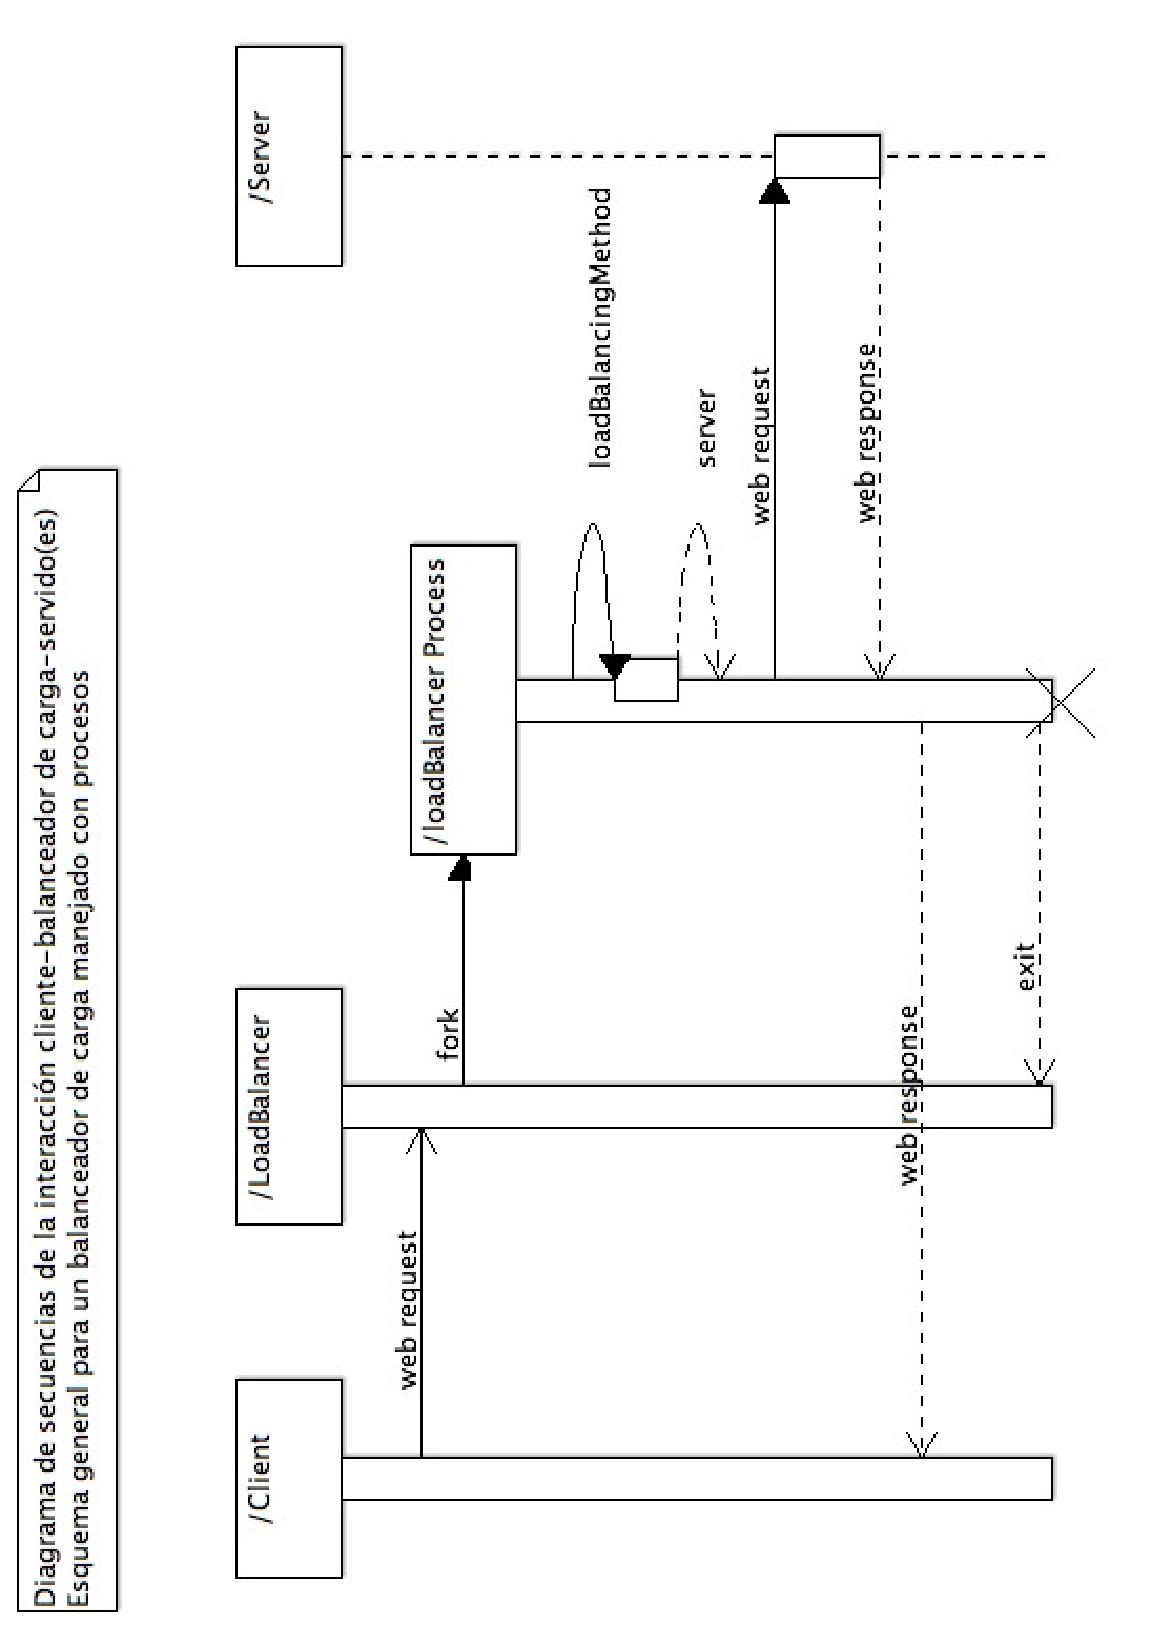
\includegraphics{diagramas/SequenceDiagram2.jpeg} 
%   \caption{example caption}
%   \label{fig:example}
%\end{figure}

%\begin{figure}[htbp] %  figure placement: here, top, bottom, or page
%   \centering
%   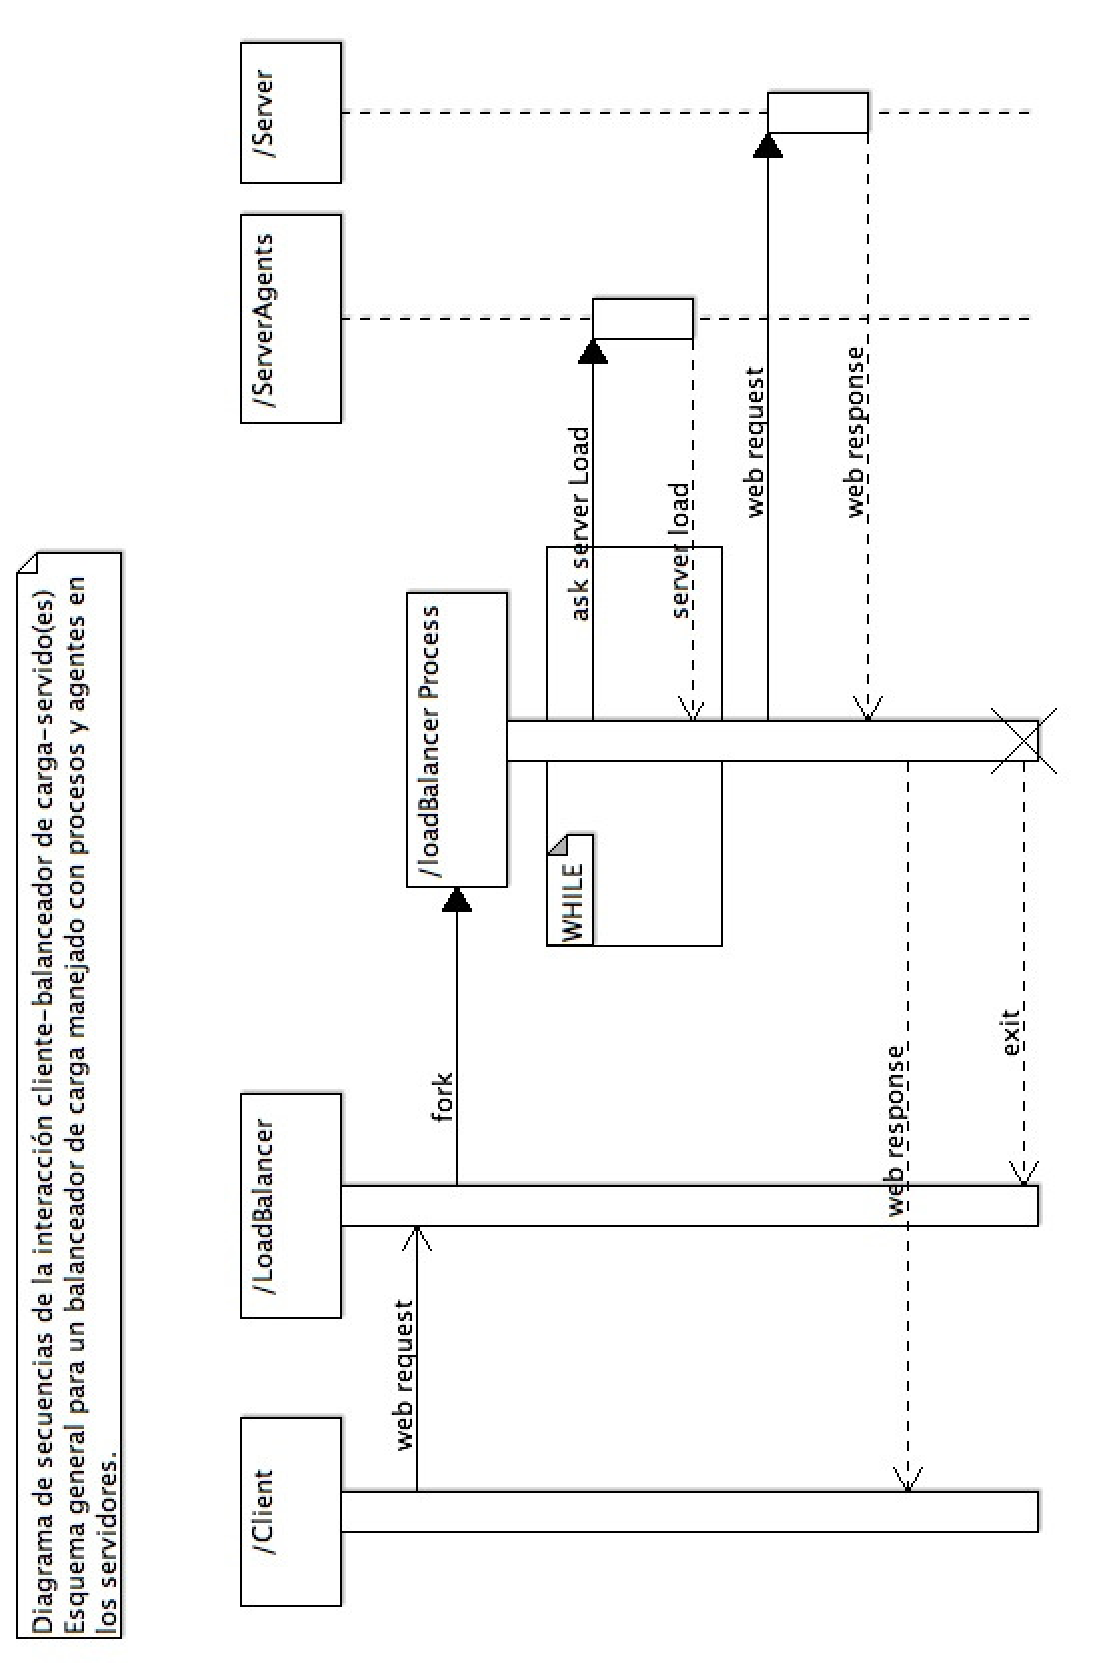
\includegraphics[width=2in]{diagramas/SequenceDiagramAgents2.jpeg} 
%   \caption{example caption}
%   \label{fig:example}
%\end{figure}
\newpage
%\begin{figure}[p]
%\centering
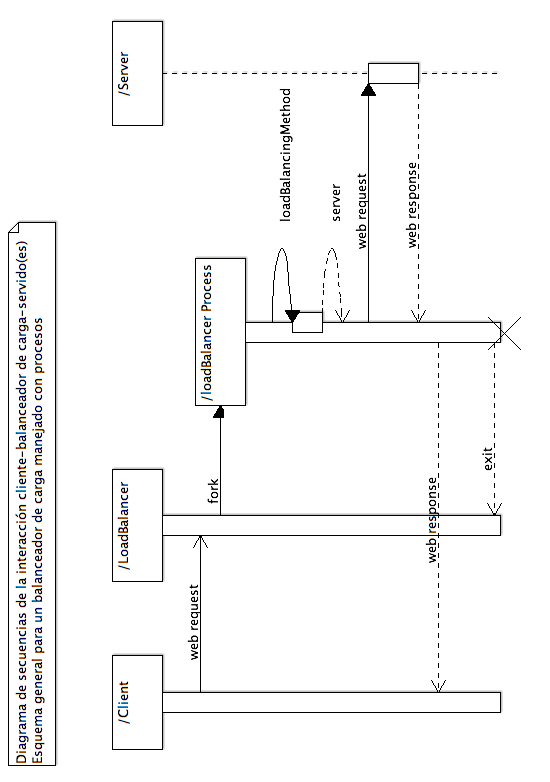
\includegraphics{diagramas/SequenceDiagram2.png}
%\caption{Some graph}
%\label{fig:graph}
%\end{figure}
\newpage
%\begin{figure}[htp]
%\centering
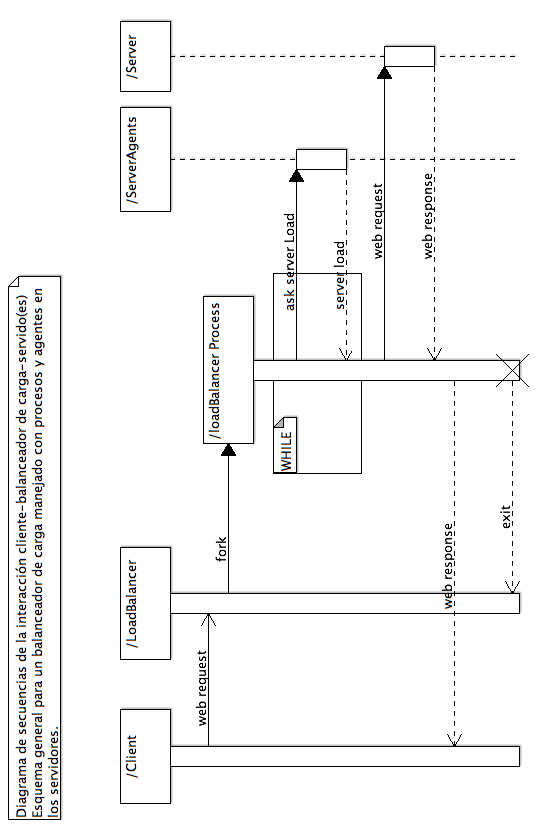
\includegraphics{diagramas/SequenceDiagramAgents2.png}
%\caption{Some graph}
%\label{fig:graph}
%\end{figure}

\section{Máquina de estado finito}
	 \begin{figure}[ht]
        \centering
        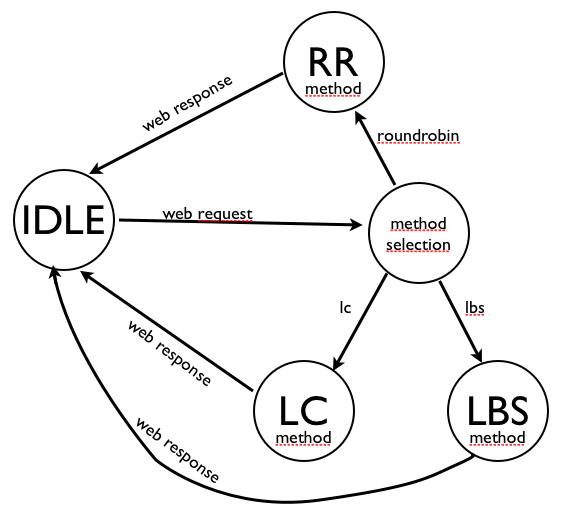
\includegraphics[scale=0.45]{diagramas/auto1.png}
        %\caption{}
      \end{figure}
      
       \begin{figure}[ht]
        \centering
        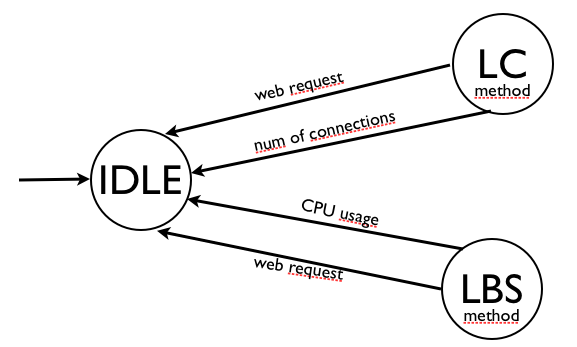
\includegraphics[scale=0.45]{diagramas/auto2.png}
        %\caption{}
      \end{figure}
	
\section{Pseudocódigos de los métodos}

	En todos los métodos se espera leer un arreglo con las direcciones de servidores que estará contenida en un archivo de configuración.
	\begin{itemize}
	\item Round Robin.
		%seudocódigo Round Robin

$\vartriangleright$ Idea: Round Robin es el método más sencillo, ya que simplemente lleva la cuenta de cuál fue el último servidor al cual se envió
petición y en base a eso envía al siguiente en la lista. La implementación se basa en un contador que se incrementa y se le aplica el módulo con
el número de servidores.\\
\begin{verbatimtab}[\myTabs]

RoundRobin
read( servers_array )
	num_servers = length( servers_array )
	server_no = 0
	
	while incoming_connection
		fork
			read( server_no )
			connect2( server_array[server_no] )
			server_no = server_no + 1
			server_no = server_no \% num_servers
			write( server_no )
		exitfork
	endwhile

endRoundRobin\\
\end{verbatimtab}\\


	\item Menor número de conexiones.
		$\triangle$ Primera aproximación a este método.
		%seudocódigo para el menor número de conexiones

$\triangle$ Idea: Este método se basa en una tabla que guarda el número de conexiones activas que tiene cada servidor, y entrega la nueva conexión
al servidor que tenga el menor número.\\

\begin{verbatimtab}[\myTabs]

LeastConnection
	read( server_array )
	connections_array
	
	while incoming_connection
		fork
			read( connections_array )
			index = lower_value( connections_array )
			if( connect2( server_array[index] ) )
				connections_array[index] ++
				write( connections_array )
				write( index )
			endif
		exitfork
		read( connections_array )
		read( index )
		connections_array[index] --
		write( connections_array )
	endwhile

endLeastConnection\\

\end{verbatimtab}\\


		$\triangle$ Aproximación definitiva a este método.
		%agente de servidor ocupado

$\vartriangleright$ Idea: Esta implementación requiere de la presencia de un agente en cada servidor que se encargará de enviar básicamente
la información sobre el número de conexiones TCP activas para que el método pueda enviar la conexión al servidor que se encuentre con menos de
este trabajo en el momento que se requiera.

\begin{verbatimtab}[\myTabs]

LeastConnections2
	read (agents_array )
	read( servers_array )
	
	while incoming_connection
		fork
			good_server = get_tcps(agent_array[0])
			it=1
			server_no
			while i < length( agents_array )
				server_tcps=get_tcps(agent_array[it])
				if ( server_tcps < good_server )
					server_no = it
				endif
			
			it = it + 1
			endwhile
			connect2( server_array[server_no] )
		exitfork
	endwhile
	
endLeastConnections2

\end{verbatimtab}
	\item Carga en servidor.
		%agente de servidor ocupado

$\vartriangleright$ Idea: Esta implementación requiere de la presencia de un agente en cada servidor que se encargará de enviar básicamente
la información sobre las cargas del procesador para que el método pueda enviar la conexión al servidor que se encuentre menos ocupado en el
momento que se requiera.\\

\begin{verbatimtab}[\myTabs]

ServerLoad
	read (agents_array )
	read( servers_array )
	
	while incoming_connection
		fork
			good_server = get_load(agent_array[0])
			it=1
			server_no
			while i < length( agents_array )
				server_load=get_load(agent_array[it])
				if ( server_load < good_server )
					server_no = it
				endif
			
			it = it + 1
			endwhile
			connect2( server_array[server_no] )
		exitfork
	endwhile
	
endServerLoad\\

\end{verbatimtab}\\


	\item Método del grupo.
		$\vartriangleright$ La idea sobre la cual se basa es un principio probabilista muy simple si un servidor cualquiera es capaz de dar un response a un
request simple, mucho mas rápido que los otros, existe una posibilidad mucho mayor, de que se  comporte mejor para un request en general,
es decir es una especie de look a head por medio del cual definimos un favorito.\\

\begin{verbatimtab}[\myTabs]
heuristica()
best <- MAX
for i <- 0 to servers
  do evaluate i
    if i better than best
      then best <- i


evaluate()
  time <- 0
  while socket sin respuesta
    time <- time +1
\end{verbatimtab}\\


	\end{itemize}
	
	$\triangle$ PS: En los seudo códigos se puede ver que en muchos pasos se debe escribir y leer información, esto se debe a que mediante el uso
	de procesos que lo que hacen es una copia idéntica y no tendría sentido usar una variable para manejar la información porque esta no podría ser
	vista por los otros procesos.

\section{Arquitectura del sistema}
	La arquitectura consiste en siempre tener un proceso que sirva de listener, y que cada vez que un cliente que se intente conectar, el listener haga fork(),
para así siempre tener el proceso en el puerto deseado, y que simplemente sea un nuevo proceso que se encargue de manejar la petición. Ahora en el
proceso hijo no hace falta listener por lo que se libera ese recurso, ahora en los procesos hijos se debe seleccionar por algún método en particular uno
de los back-end, una vez escogido uno de estos, establecemos la conexión con el back-end en el mismo proceso y en teoría solo bastaría con transferir
los buffers entre los sockets, y al final cerrar las conexiones y cerras los procesos.\\



\section{Pruebas}
	Todas las pruebas del balanceador de cargas por Round Robin fueron a pequeña escala, el ambiente de pruebas fueron dos portátiles, donde cada
portátil corría dos servidores web con páginas de inicio de desarrollos en blanco de Ruby on Rails y drupal. Una de las máquinas ejecutaba el
balanceador de cargas y desde las dos se hacían peticiones que recibía el balanceador de carga.\\

Las máquinas corrieron con estas configuraciones:
Portátil 1: IP:10.0.1.5
\begin{center}
\begin{tabular}{ l r }
Aplicación & Puerto \\ \hline
ROR &  4000 \\
Drupal  & 5000\\
LoadBalancer & 80 \\
\end{tabular}
\end{center}
Esta máquina realiza las peticiones mediante un explorador Firefox.\\ \\

Portátil 2: IP:10.0.1.4
\begin{center}
\begin{tabular}{ l r }
Aplicación & Puerto \\ \hline
ROR  & 4000 \\
Drupal  & 5000\\
\end{tabular}
\end{center}
Esta máquina realiza las peticiones mediante un explorador Safari.\\ \\



Las pruebas realizadas al método de balanceo LBS que requiere un agente en el servidor se realizó con dos máquinas, un portátil y un servidor.
En las dos máquinas se corrió una aplicación en blanco, para el servidor se corrió en Apache y en el portátil una aplicación en blanco en Ruby on Rails
con servidor Webrick.\\
La prueba consistió en correr un ``fork bomb'' con el siguiente código en C:

\begin{lstlisting}[language=C]
int main()
{
 int i=10000000;
 while(i--)
  fork();
 return 0;
}
\end{lstlisting}

El cual al cabo de unos segundos eleva la carga del procesador del servidor a un punto en el que podíamos observar cuando dejaba de enviar las
peticiones al servidor y cambiaba al portátil, también después de detener la ``bomba de procesos'' veíamos como el balanceador enviaba las nuevas
peticiones al servidor.\\


	
\section{Conclusiones}
	El aspecto más interesante de esta práctica podría ser el hecho de que había que llegar a otro nivel de abstracción para comprender todo el
funcionamiento de las aplicaciones para redes y web en este caso. Fue muy claro que las dificultades se presentan dependiendo del lenguaje en 
que se decida trabajar, puesto que el manejo de sockets y esquemas requeridos para desarrollos en telemática requieren tener mayor dominio en
lenguajes como C o C++, mientras que hay otros que proveen todas las herramientas para que el trabajo con estas nuevas funciones sea casi
transparente.
A nivel de la se necesitó investigar conceptos que no se habían visto anteriormente en la carrera, todo el manejo de procesos, hilos y segmentación en
cuanto a las peticiones fueron grandes retrasos en el desarrollo de la práctica.
	
\begin{thebibliography}{1}

\bibitem{GitHub}
\newblock{GitHub$^{\rm TM}$ - Social codign}\\
\newblock {\em http://github.com/sarcilav/loadbalancer20092} \\
\newblock {\em http://github.com/sergiobuj/loadbalancer20092} \\
\newblock Sitios donde se encuentra todo el desarrollo y código e la práctica.

\end{thebibliography}


\end{document}
